\renewcommand*{\arraystretch}{1.1}

\subsection*{Interactive / short / 4}
\label{section:interactive-short-read-04}

% change \emph{} to use sans-serif font
\let\oldemph\emph
\renewcommand{\emph}[1]{{\footnotesize \sf #1}}

\renewcommand{\currentQueryCard}{4}
\marginpar{
	\raggedleft
	\vspace{0.22ex}

	\queryRefCard{interactive-short-read-01}{IS}{1}\\
	\queryRefCard{interactive-short-read-02}{IS}{2}\\
	\queryRefCard{interactive-short-read-03}{IS}{3}\\
	\queryRefCard{interactive-short-read-04}{IS}{4}\\
	\queryRefCard{interactive-short-read-05}{IS}{5}\\
	\queryRefCard{interactive-short-read-06}{IS}{6}\\
	\queryRefCard{interactive-short-read-07}{IS}{7}\\
}


\noindent\begin{tabularx}{\queryCardWidth}{|>{\queryPropertyCell}p{\queryPropertyCellWidth}|X|}
	\hline
	query & Interactive / short / 4 \\ \hline
%
	title & Message Content \\ \hline
%
	pattern & \multicolumn{1}{c|}{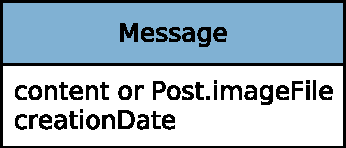
\includegraphics[scale=\patternscale,margin=0cm .2cm]{patterns/interactive-short-read-04}} \\ \hline
%
	desc. & Given a Message, retrieve its content and creation date.
 \\ \hline
%
	
		params &
		\innerCardVSpace{\begin{tabularx}{\attributeCardWidth}{|>{\paramNumberCell}c|>{\varNameCell}M|>{\typeCell}m{\typeWidth}|Y|} \hline
		$\mathsf{1}$ & Message.id
 & ID
 &  \\ \hline
		\end{tabularx}}\innerCardVSpace \\ \hline
	
%
	
		result &
		\innerCardVSpace{\begin{tabularx}{\attributeCardWidth}{|>{\resultNumberCell}c|>{\varNameCell}M|>{\typeCell}m{\typeWidth}|>{\resultOriginCell}c|Y|} \hline
		$\mathsf{1}$ & Message.creationDate & ID & R &
				 \\ \hline
		$\mathsf{2}$ & Message.content or Post.imageFile & String & R &
				 \\ \hline
		\end{tabularx}}\innerCardVSpace \\ \hline
	
%
	%
	%
	%
	%
\end{tabularx}
\queryCardVSpace

% change \emph back to the old one
\let\emph\oldemph